\chapter{Modélisation}

Dans cette section, nous avons testé plusieurs algorithmes de classification afin de prédire la probabilité d’admission des candidats. 
Les modèles utilisés sont : \textbf{SVM (SVC)}, \textbf{Arbre de décision}, \textbf{Forêt aléatoire}, \textbf{Régression logistique} et \textbf{K plus proches voisins (KNN)}. 
Pour chaque modèle, nous avons appliqué une normalisation des données avec \texttt{StandardScaler} et utilisé un pipeline pour enchaîner les étapes.

\section{Évaluation des modèles}
Chaque modèle a été entraîné sur $80\%$ des données et testé sur $20\%$. Les métriques utilisées pour comparer les performances sont :
\begin{itemize}
    \item \textbf{Accuracy} : proportion de prédictions correctes.
    \item \textbf{Precision} : proportion de vrais positifs parmi les positifs prédits.
    \item \textbf{Recall} : proportion de vrais positifs correctement détectés.
    \item \textbf{F1-score} : moyenne harmonique entre précision et rappel.
\end{itemize}

\section{Résultats comparatifs}
Les performances globales sont résumées dans le tableau suivant :

\begin{table}[H]
\centering
\begin{tabular}{lcccc}
\hline
\textbf{Modèle} & \textbf{Accuracy} & \textbf{Précision} & \textbf{Rappel} & \textbf{F1-score} \\
\hline
SVC & 0.90 & 0.94 & 0.91 & 0.92 \\
Arbre de décision & 0.76 & 0.82 & 0.82 & 0.82 \\
Forêt aléatoire & 0.87 & 0.89 & 0.93 & 0.91 \\
Régression logistique & 0.87 & 0.92 & 0.88 & 0.90 \\
KNN & 0.87 & 0.92 & 0.88 & 0.90 \\
\hline
\end{tabular}
\caption{Comparaison des performances des différents modèles.}
\end{table}

\section{Courbes d'apprentissage}
Pour mieux comprendre le biais et la variance de chaque modèle, nous avons tracé les courbes d'apprentissage. Ces dernières montrent l’évolution de la performance en fonction de la taille de l’échantillon d’entraînement.

\begin{figure}[H]
    \centering
    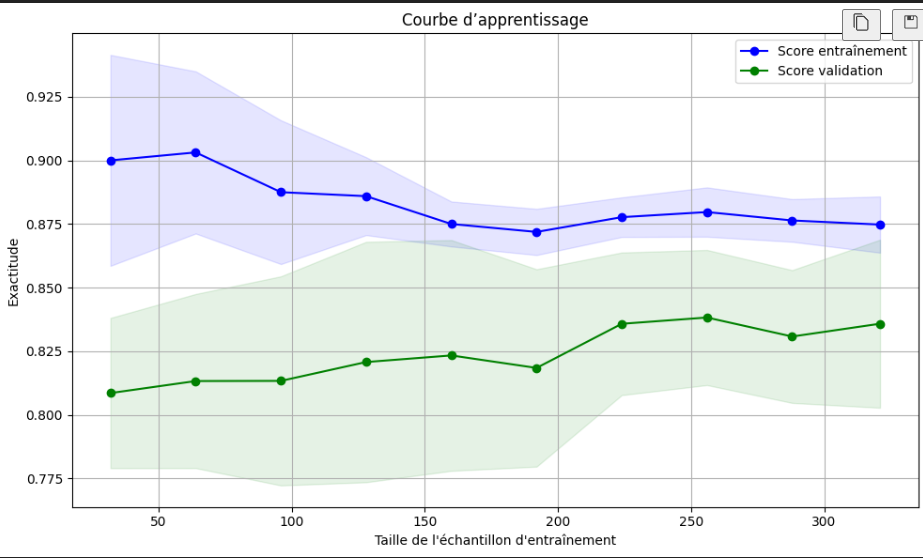
\includegraphics[width=0.7\textwidth]{figures/learning_curve_svc.png}
    \caption{Courbe d’apprentissage pour SVC.}
\end{figure}

\begin{figure}[H]
    \centering
    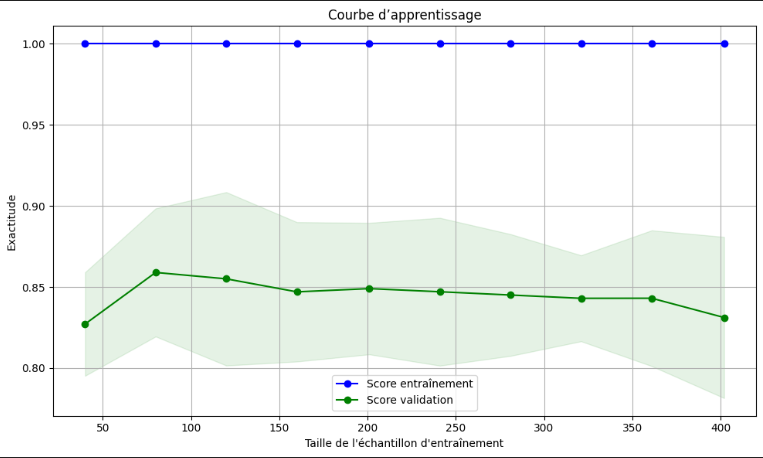
\includegraphics[width=0.7\textwidth]{figures/learning_curve_rf.png}
    \caption{Courbe d’apprentissage pour Forêt aléatoire.}
\end{figure}

\begin{figure}[H]
    \centering
    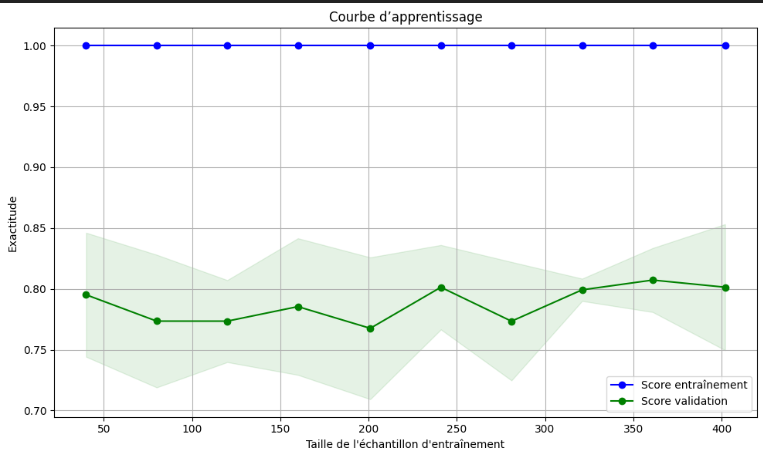
\includegraphics[width=0.7\textwidth]{figures/learning_curve_dtc.png}
    \caption{Courbe d’apprentissage pour Arbre de décision.}
\end{figure}

\begin{figure}[H]
    \centering
    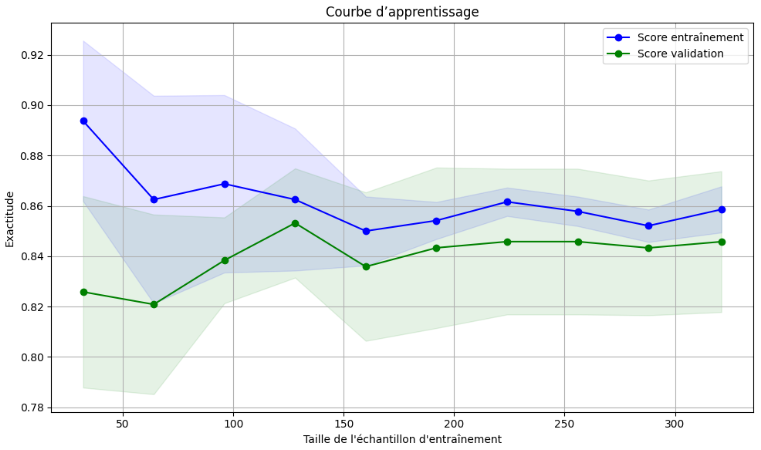
\includegraphics[width=0.7\textwidth]{figures/learning_curve_lr.png}
    \caption{Courbe d’apprentissage pour Régression logistique.}
\end{figure}

\begin{figure}[H]
    \centering
    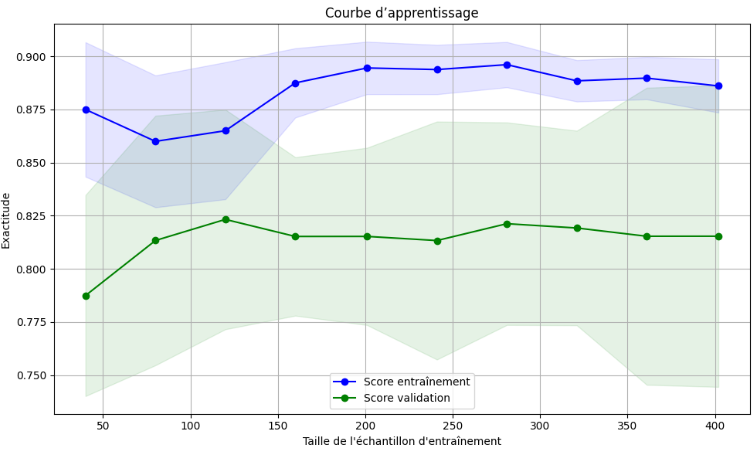
\includegraphics[width=0.7\textwidth]{figures/learning_curve_knn.png}
    \caption{Courbe d’apprentissage pour KNN.}
\end{figure}

\section{Discussion}
L’analyse comparative montre que : 
\begin{itemize}
    \item Le modèle \textbf{SVC} obtient la meilleure performance globale avec un F1-score de 0.92, grâce à une bonne précision et un bon rappel.
    \item Les modèles \textbf{Forêt aléatoire} et \textbf{KNN} présentent des résultats proches (accuracy de 0.87 et F1-score de 0.90). 
    \item L’\textbf{arbre de décision}, en revanche, a un score plus faible (accuracy 0.76), et tend à sur-apprendre les données d’entraînement (overfitting).
    \item La \textbf{régression logistique} se démarque car, contrairement aux modèles comme l’arbre de décision, la forêt aléatoire ou KNN qui mémorisent fortement les données, elle parvient à \textbf{apprendre une véritable relation généralisable entre les variables et la probabilité d’admission}. 
\end{itemize}

Ainsi, même si SVC donne les meilleurs résultats en termes de F1-score, la régression logistique apparaît comme un modèle plus robuste et interprétable pour ce type de problématique. Elle a donc été retenue et sauvegardée pour de futures prédictions.
